\documentclass[12pt]{report}
\usepackage[a4paper]{geometry}
\usepackage{fancyhdr}
\pagestyle{fancy}
\fancyhead[c]{}
\fancyhead[l]{\thechapter}
\fancyhead[r]{\thesection}

\fancyfoot[l]{}
\fancyfoot[c]{\thepage}
\fancyfoot[r]{}

\usepackage{math-packages}
\usepackage{math-environments}
\usepackage{math-macros}
\usepackage{tikz}

\usepackage{fontspec}
\setmainfont{Gill Sans Light}

\usepackage[citestyle=alphabetic,
% bibstyle=authortitle,
backend=biber]{biblatex}
\addbibresource{bibliography.bib}

\newenvironment{note}{\begin{bluebox}}{\end{bluebox}}
\newenvironment{warning}{\begin{redbox}}{\end{redbox}}



\title{Mathematics}
\author{James Leslie}
\date{\today}
\begin{document}
\maketitle
\tableofcontents

\part{Pre-Honours Courses}\label{part:pre-honours-courses}
\chapter{Introduction to Group Theory}\label{cha:intr-group-theory}
Introduction to Group Theory was my first ``real'' taste of algebra at university. It was half of the course Fundamental of Pure Mathematics, the other half being an introduction to real analysis. I took this course in the second semester of my second year in 2015, and the group theory part was taught by \href{https://www.maths.gla.ac.uk/~mwemyss/}{Michael Wemyss}. This chapter is based off the notes~\cite{wemyss2015grouptheory}.

\section{Groups and Symmetries}
The study of any area of pure mathematics needs to be well motivated. Group theory is really the study of automorphisms. This becomes quite tangible when applied to concrete objects such as graphs, whose automorphisms are symmetries.

\begin{definition}\cite[Definition 1.1.1]{wemyss2015grouptheory}\label{def:intr-group-theory:graph}
  A \indx{graph} is a finite set of vertices, with at most one edge between any two vertices. There are no self edges allowed.
\end{definition}

\begin{example}
  The following are examples of graphs.

  % TODO: Add more tikz graphs and tidy up.
  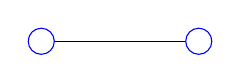
\begin{tikzpicture}
    \node[shape=circle, draw=blue] (A) at (-1,0) {};
    \node[shape=circle, draw=blue] (B) at (1,0) {};

    \path [-] (A) edge (B);
  \end{tikzpicture}
\end{example}

\begin{definition}\cite[Definition 1.1.3]{wemyss2015grouptheory}
  A symmetry of a graph is a bijection \(f : V \to V\) on such that \(f(v_{1})\) and \(f(v_{2})\) are joined by an edge if and only if \(v_{1}\) and \(v_{2}\) are joined by an edge.
\end{definition}

\begin{example}
  Determine all the symmetries of the following graph:

  \begin{centre}
    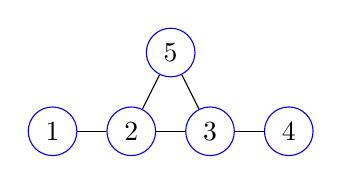
\begin{tikzpicture}
      \node[shape=circle, draw=blue] (1) at (0,0) {1};
      \node[shape=circle, draw=blue] (2) at (1,0) {2};
      \node[shape=circle, draw=blue] (3) at (2,0) {3};
      \node[shape=circle, draw=blue] (4) at (3,0) {4};
      \node[shape=circle, draw=blue] (5) at (1.5,1) {5};

      \path [-]  (1) edge (2);
      \path [-]  (2) edge (3);
      \path [-]  (3) edge (4);
      \path [-]  (2) edge (5);
      \path [-]  (3) edge (5);
    \end{tikzpicture}
  \end{centre}

  Let \(f\) be an arbitrary symmetry. By definition, \(f\) must preserve the valency of vertices. As vertex 5 is the only vertex of valency 2, we must have that \(f(5) = 5\). Since vertices 2 and 3 are the only vertices of valency 3, \(f\) can either fix them, or swap them.
  \begin{enumerate}
    \item Suppose they are fixed. Then \(f\) fixes both 1 and 4 as \(f(1)\) has valency 1 and must be connected to \(f(2) = 2\), hence \(f(1) = 1\). A similar argument applies to vertex 4. The completes the case where \(f\) fixes vertex 2 and 3.
    \item Suppose they are swapped. Then \(f(1) = 4\), as \(f(1)\) must have valency 1 and be connected to \(f(3) = 3\). Likewise, \(f(4) = 1\).
  \end{enumerate}

  Hence there are exactly two symmetries.
\end{example}

\begin{note}
  The definition of a symmetry is not dependent on the embedding of the graph in the plane. It is easy to visually inspect a graph and gain an intuition about the symmetries, but a formal proof requires one to be more precise.
\end{note}


\section{Groups and examples}

\begin{definition}\label{def:intro-to-group-theory:group}
  A \indx{group} \(G\) is a set \(G\) equipped with a binary operation \(* : G \times G \to G\), a unary operation \((-)^{-1}: G \to G\), and an identity element \(e \in G\) such that the following properties hold:

  \begin{enumerate}
    \item \(*\) is associative (\((g * h) * j = g * (h * j)\));
    \item \(e * g = g = g * e\), for all \(g \in G\);
    \item \(g * g^{-1} = e = g^{-1} * g\).
  \end{enumerate}

  The \indx{order} of a group \(G\), denotes \(|G|\) is the cardinality of the underlying set.
\end{definition}

\begin{example}
  The automorphisms of an object (i.e the symmetries of a graph) form a group.
\end{example}

\begin{example}
  The integers \(\Z\) form a group under addition.
\end{example}

\begin{example}
  \(S_{n}\), the \index{symmetric group} on \(n\) elements is the set of permutations of \(\{1, \ldots, n\}\). It is a group under composition.

  We typically use cycle notation \((123)(12): S_{3} \to S_{3}\), where \((123)\) means the permutation sending 1 to 2, 2 to 3 and 3 to 1. Two bracket cycles next to each other for a permutation by composition.
\end{example}

\begin{example}

\end{example}
% TODO Add more examples

\section{First properties of groups}\label{sec:intro-to-group-theory:first-prop-groups} % TODO

\section{Lagrange's Theorem and applications}\label{sec:intro-to-group-theory:lagrange} % TODO

\section{Homomorphisms and isomorphisms}\label{sec:intro-to-group-theory:homomorphisms} % TODO

\section{Group actions}\label{sec:intro-to-group-theory:group-actions} % TODO

\section{Symmetric and alternating groups}\label{sec:intro-to-group-theory:symmetric-alternating-groups} % TODO

\section{Conjugacy and normal subgroups}\label{sec:intro-to-group-theory:conjugacy-normal-subgroups} % TODO











\chapter{Introduction to Real Analysis}\label{cha:intr-real-analys}
\chapter{Calculus}\label{cha:calculus}
\chapter{Probability with Applications}\label{cha:prob-with-appl}
\chapter{Statistics}\label{cha:statistics}

\part{Honours Courses}
\chapter{Honours Algebra}\label{cha:honours-algebra}
\chapter{Honours Analysis}\label{cha:honours-analysis}
\chapter{Complex Variables}\label{cha:complex-variables}
\chapter{Honours Differential Equations}\label{cha:hono-diff-equat}

\part{Post-honours Courses}\label{part:post-honours-courses}
\chapter{Geometry}\label{cha:geometry}
\chapter{Combinatorics and Graph Theory}\label{cha:comb-graph-theory}
\chapter{Commutative Algebra}\label{cha:commutative-algebra}
\chapter{Essentials in Analysis and Probability\label{cha:essent-analys-prob}}
\chapter{Introduction to Number Theory}\label{cha:intr-numb-theory}
\chapter{General Topology}\label{cha:general-topology}
\chapter{Algebraic Topology}\label{cha:algebraic-topology}
\chapter{Group Theory}\label{cha:group-theory}
This is a continuation of the Group Theory learned in Chapter~\ref{cha:intr-group-theory}





\chapter{Galois Theory}\label{cha:galois-theory}
\chapter{Linear Analysis}\label{cha:linear-analysis}
\chapter{Fourier Analysis}\label{cha:fourier-analysis}

\part{Graduate Studies}\label{part:graduate-studies}

\chapter{Algebraic Geometry}\label{cha:algebraic-geometry}
\chapter{Complex Algebraic Curves}\label{cha:compl-algebr-curv}
\chapter{Lie Algebras}\label{cha:lie-algebras}
\chapter{Quantum Information}\label{cha:quantum-information}
\chapter{Variational Calculus}\label{cha:variational-calculus}


\part{Category Theory and its Applications}\label{part:category-theory-its}
\chapter{Category Theory}\label{cha:category-theory}
\chapter{Homotopy Theory}\label{cha:homotopy-theory}
\chapter{Higher Category Theory}\label{cha:high-categ-theory}
\chapter{Multidimensional Category Theory}\label{cha:mult-categ-theory}

\printbibliography%
\end{document}
